%================================================================
\section{Appendix}\label{sec:Appendix A}
%================================================================



%----------------------------------------------------------------
\subsection{Additional Results}\label{app:additional_results}
%---------------------------------------------------------------- 

\subsubsection*{Binarized MNIST experiments}

\autoref{fig:samples_latent_dim_vanilla_vae_bmnist} shows generated samples. The left column (a, d, g) displays outputs from the MLP-VAE, the middle column (b, e, h) the DNN-VAE, and the right column (c, f, i) the Conv-VAE. The top, middle, and bottom rows shows the outcomes for 1, 20, and 100 latent dimensions, respectively. 

\begin{figure}[!htb]
\centering
\subfloat[]{{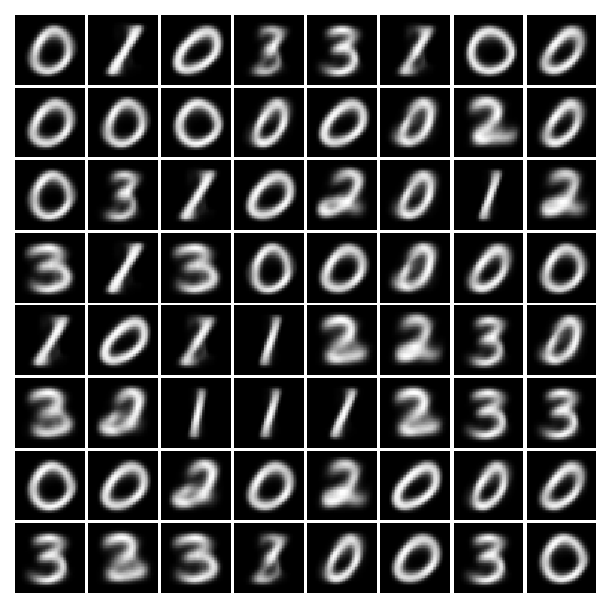
\includegraphics[scale=0.45]{latex/figures/samples_latent_dim_1_vanilla_mlp_vae_bmnist.pdf}}}
\qquad
\subfloat[]{{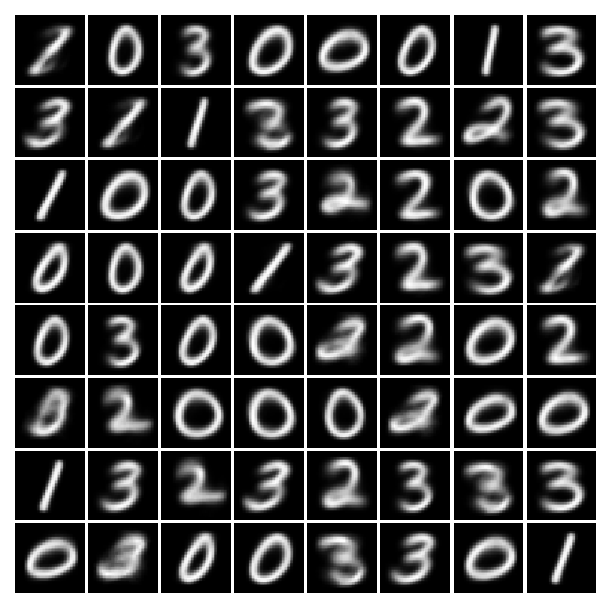
\includegraphics[scale=0.45]{latex/figures/samples_latent_dim_1_vanilla_dnn_vae_bmnist.pdf}}}
\qquad
\subfloat[]{{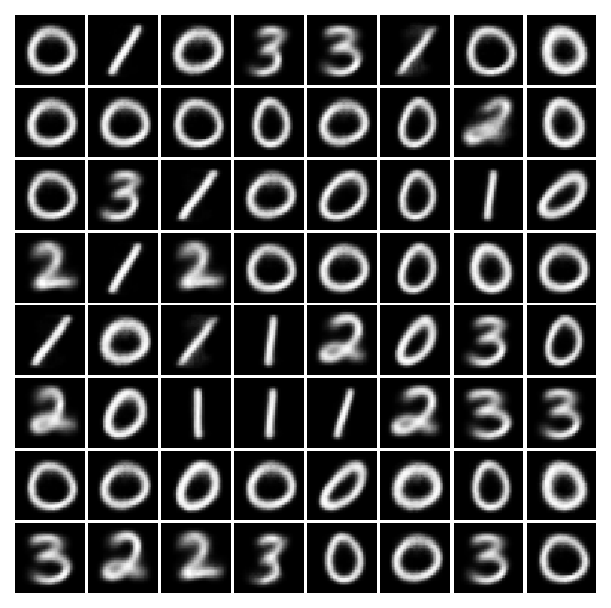
\includegraphics[scale=0.45]{latex/figures/samples_latent_dim_1_vanilla_conv_vae_bmnist.pdf}}}
\qquad
\subfloat[]{{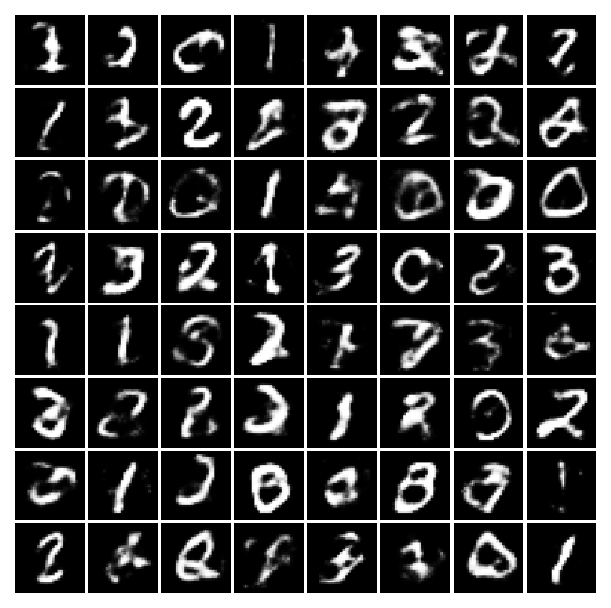
\includegraphics[scale=0.45]{latex/figures/samples_latent_dim_20_vanilla_mlp_vae_bmnist.pdf}}}
\qquad
\subfloat[]{{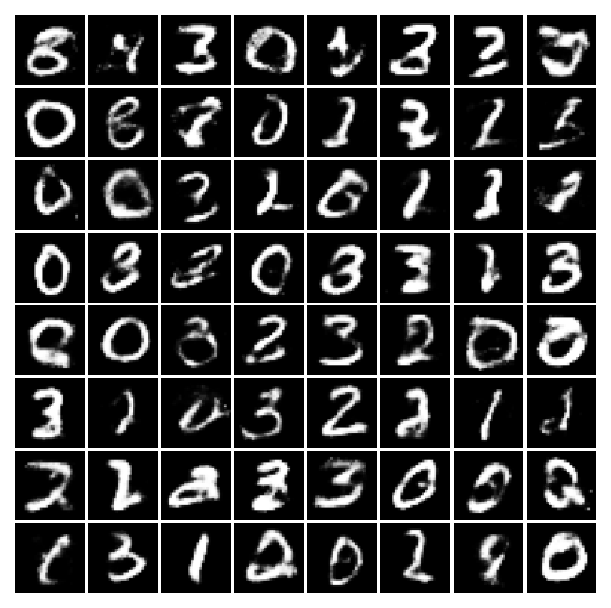
\includegraphics[scale=0.45]{latex/figures/samples_latent_dim_20_vanilla_dnn_vae_bmnist.pdf}}}
\qquad
\subfloat[]{{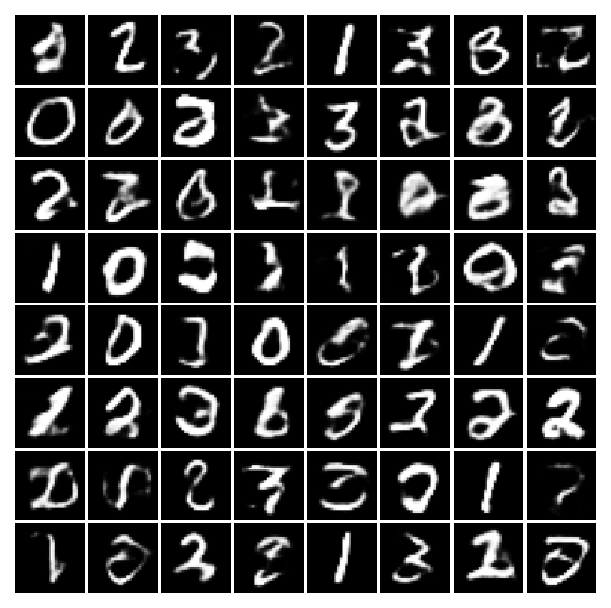
\includegraphics[scale=0.45]{latex/figures/samples_latent_dim_20_vanilla_conv_vae_bmnist.pdf}}}
\qquad
\subfloat[]{{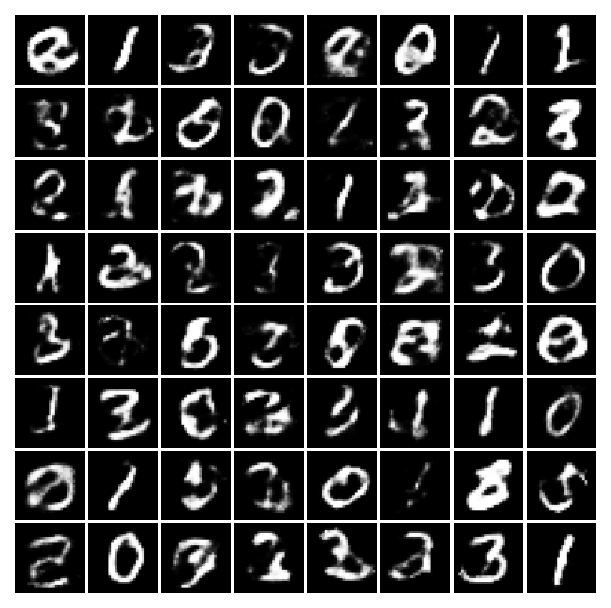
\includegraphics[scale=0.45]{latex/figures/samples_latent_dim_100_vanilla_mlp_vae_bmnist.pdf}}}
\qquad
\subfloat[]{{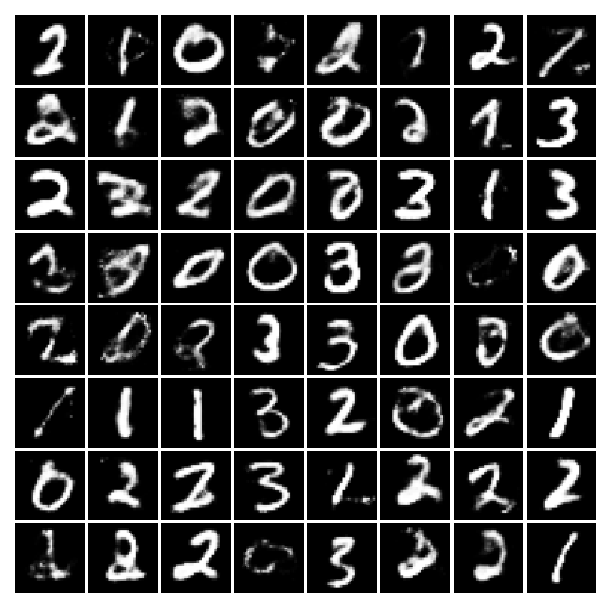
\includegraphics[scale=0.45]{latex/figures/samples_latent_dim_100_vanilla_dnn_vae_bmnist.pdf}}}
\qquad
\subfloat[]{{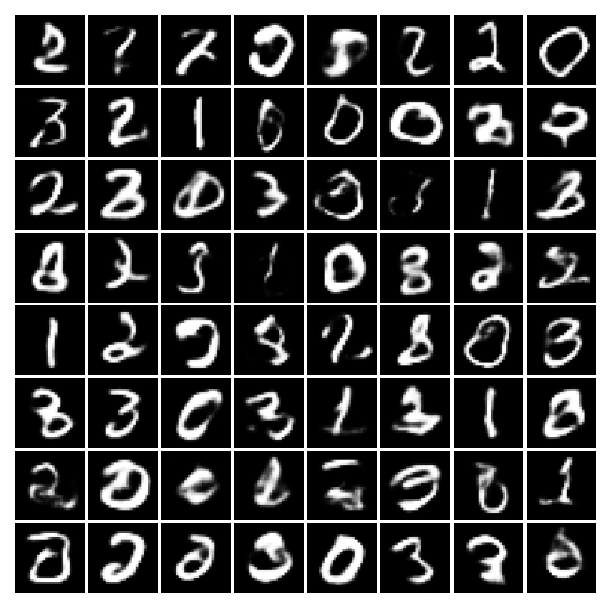
\includegraphics[scale=0.45]{latex/figures/samples_latent_dim_100_vanilla_conv_vae_bmnist.pdf}}}
\caption{Comparison of generated images with the MLP-VAE on the left, the DNN-VAE in the middle, and the Conv-VAE on the right. The top row displays generated images for 1 latent dimension, the middle row for 20 latent dimensions, and the bottom row for 100 latent dimensions.}
\label{fig:samples_latent_dim_vanilla_vae_bmnist}
\end{figure}

\subsubsection*{Neural data experiments}

%\autoref{fig:hh_mlp_vae_beta_1_z_20}

%\begin{figure}[!htb]
%\begin{center}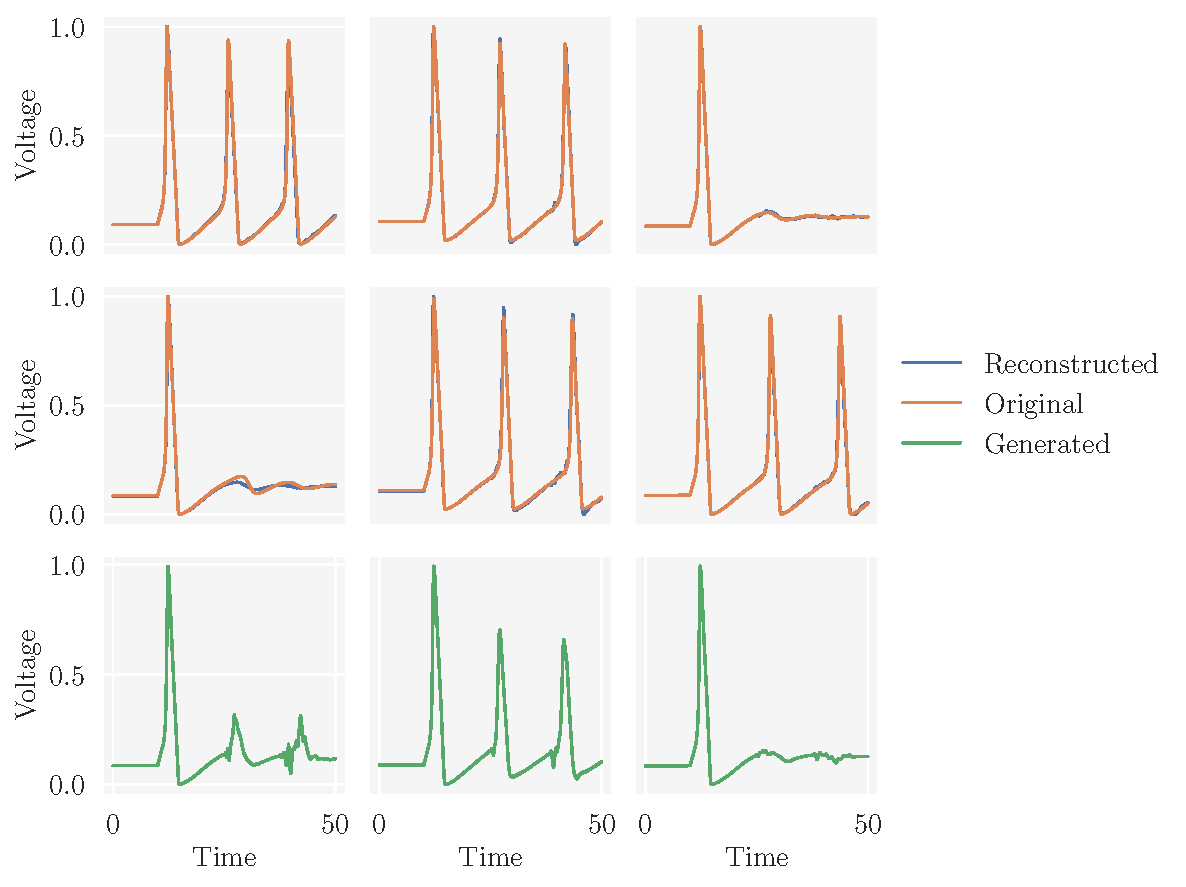
\includegraphics[scale=0.75]{latex/figures/hh_mlp_vae_beta_1_z_20.pdf}
%\end{center}
%\caption{beta 1, z 20, mlp}
%\label{fig:hh_mlp_vae_beta_1_z_20}
%\end{figure}

%\autoref{fig:hh_mlp_vae_beta_1_z_2}

%\begin{figure}[!htb]
%\begin{center}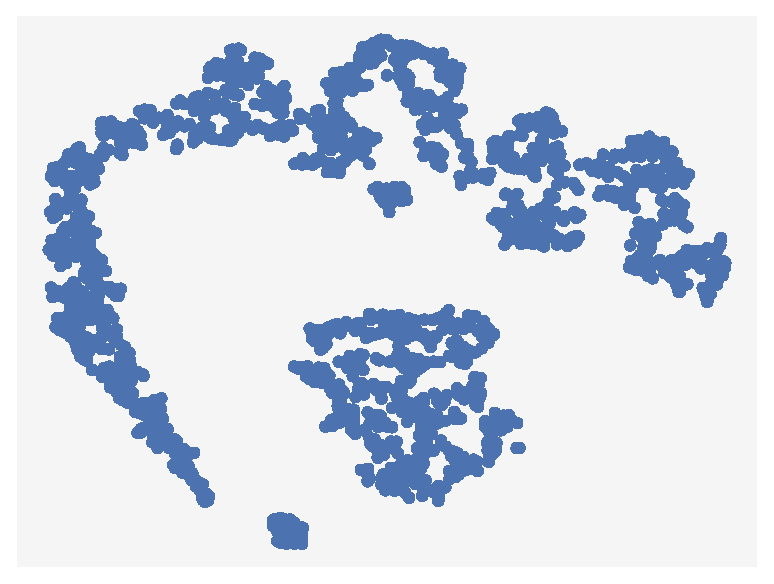
\includegraphics[scale=0.75]{latex/figures/hh_tsne_mlp_vae_beta_1_z_2.pdf}
%\end{center}
%\caption{beta 1, z 2, mlp}
%\label{fig:hh_mlp_vae_beta_1_z_2}
%\end{figure}

\autoref{fig:hh_beta_vae_tradeoff} shows the ELBO loss components after training the convolutional $\beta$-VAE on the HH dataset over 100 epochs for different latent space dimensions, $\dim(z)$. 

\begin{figure}[!htb]
\begin{center}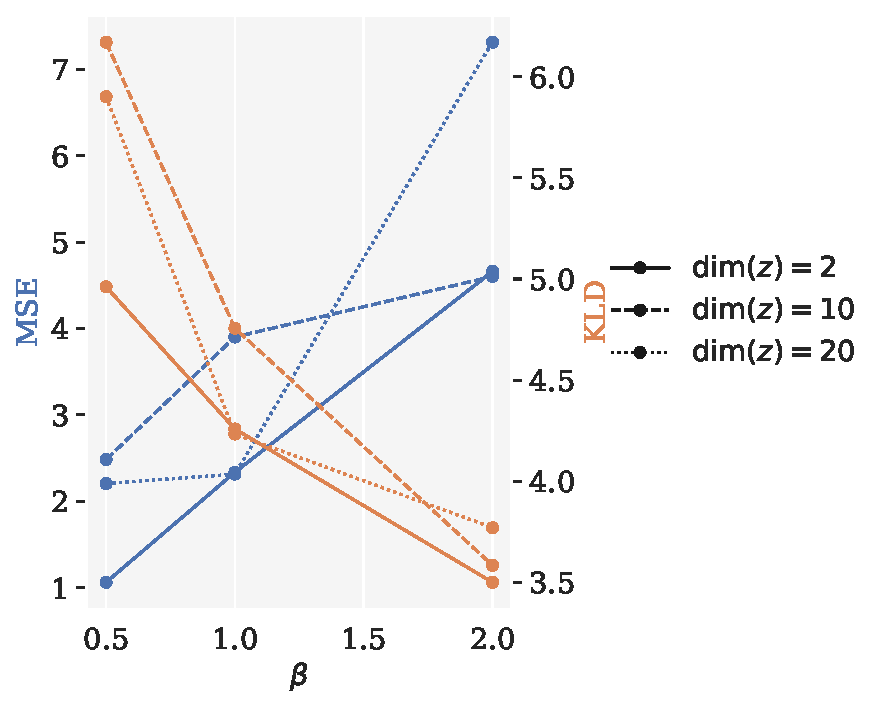
\includegraphics[scale=0.75]{latex/figures/hh_mse_kld_vs_beta_conv_vae.pdf}
\end{center}
\caption{The tradeoff between the reconstruction (MSE) and regularization (KLD) terms of the ELBO.}
\label{fig:hh_beta_vae_tradeoff}
\end{figure}

\autoref{fig:hh_conv_vae_beta_0_5} and \autoref{fig:hh_conv_vae_beta_2} are supplementary to \autoref{fig:hh_conv_vae_beta_1_z_20}, \ref{fig:hh_conv_vae_beta_1_z_10} and \ref{fig:hh_conv_vae_beta_1_z_2}, and show the convolutional $\beta$-VAE's reconstructed and generated voltage traces for $\beta = 0.5$ and $\beta=2$, respectively, with $\dim (z) = \{2, 10, 20\}$.

\begin{figure}[!htb]
\centering
\subfloat[]{{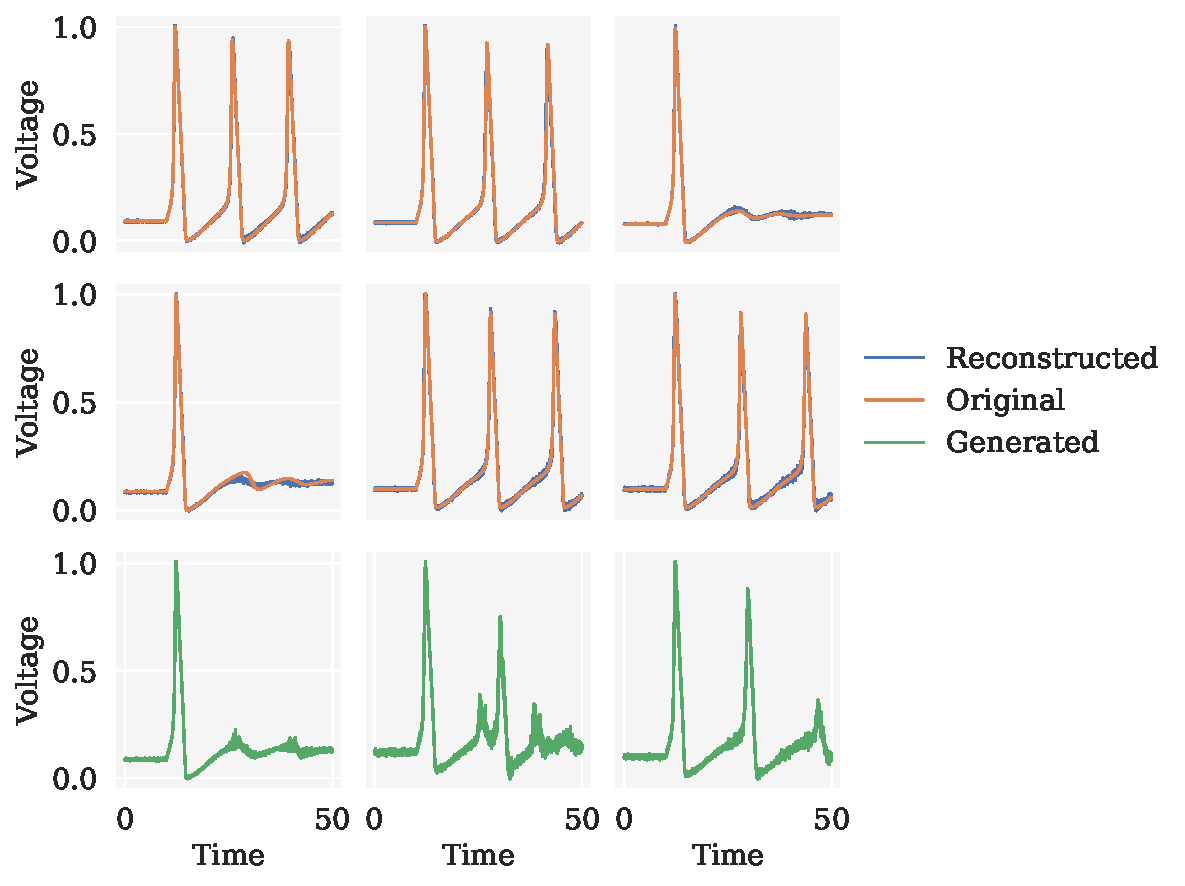
\includegraphics[scale=0.38]{latex/figures/hh_conv_vae_beta_0.5_z_2.pdf}}}
\qquad
\subfloat[]{{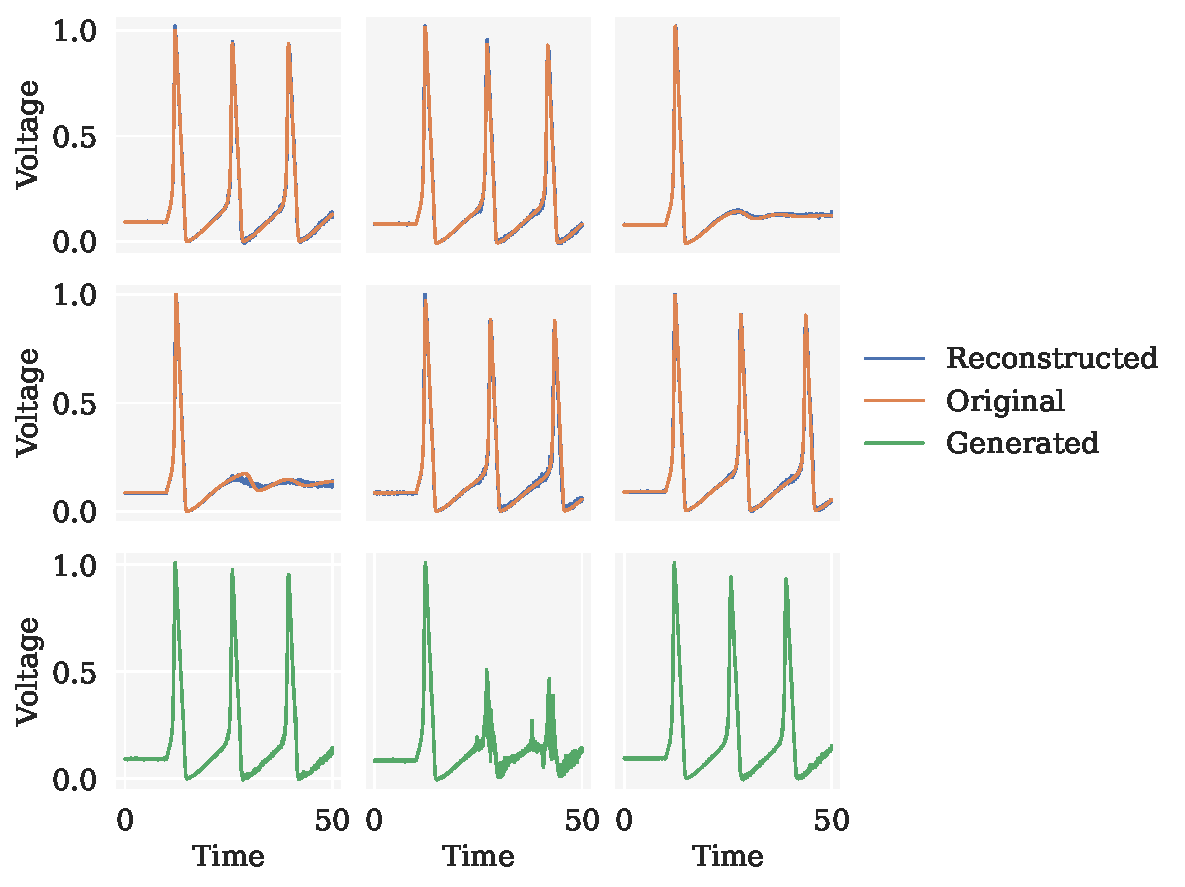
\includegraphics[scale=0.38]{latex/figures/hh_conv_vae_beta_0.5_z_10.pdf}}}
\qquad
\subfloat[]{{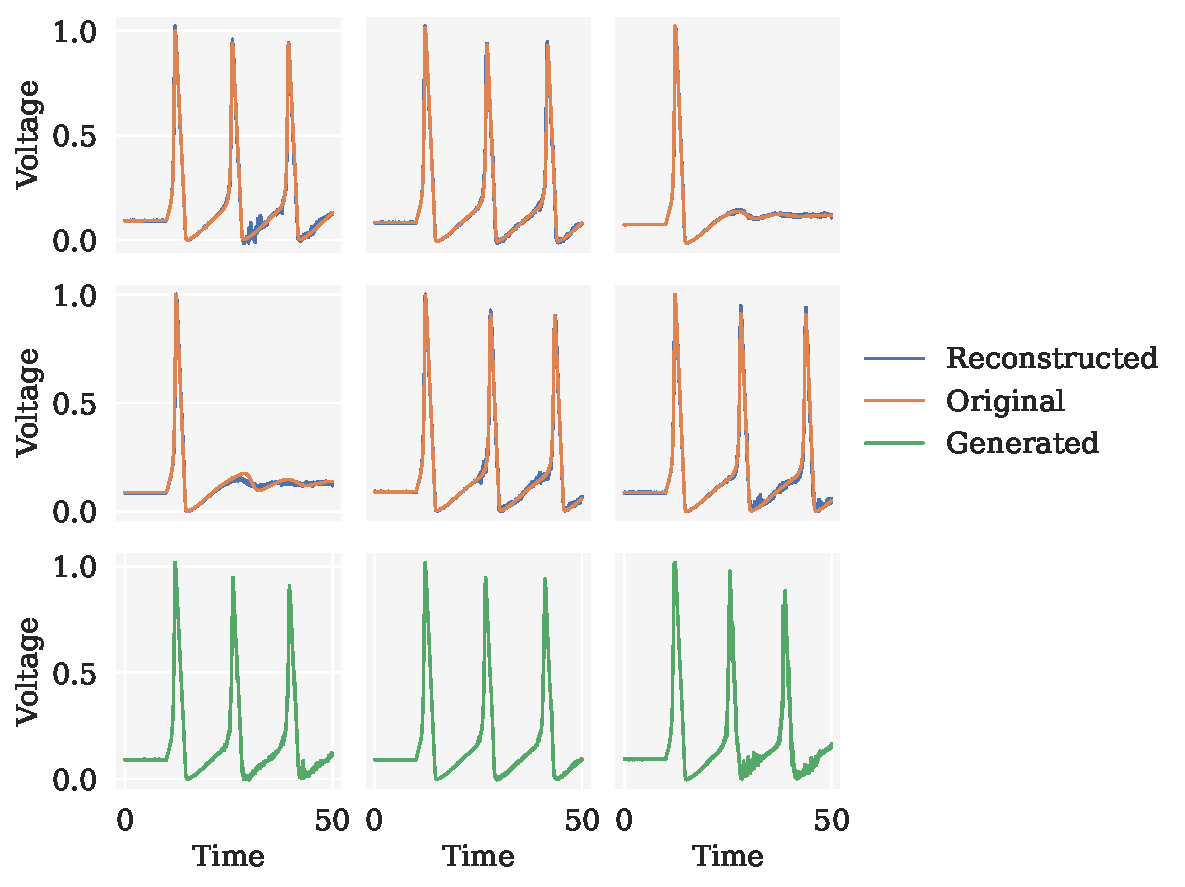
\includegraphics[scale=0.38]{latex/figures/hh_conv_vae_beta_0.5_z_20.pdf}}}
\caption{Reconstructed voltage traces overlayed with the original signals for a convolutional $\beta$-VAE with $\beta=0.5$, together with novel voltage traces generated from the latent space. The latent dimensions are (a) 2, (b), 10, (c) 20.}
\label{fig:hh_conv_vae_beta_0_5}
\end{figure}

\begin{figure}[!htb]
\centering
\subfloat[]{{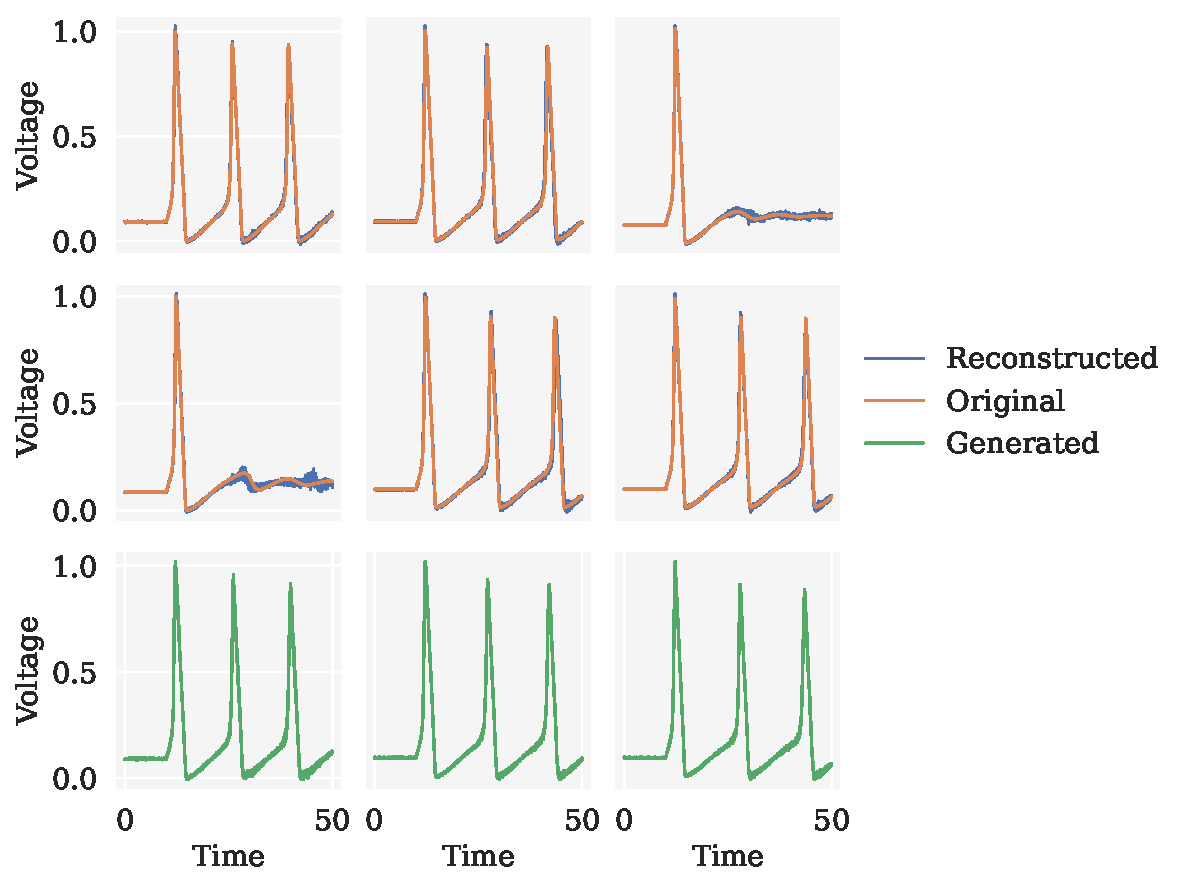
\includegraphics[scale=0.38]{latex/figures/hh_conv_vae_beta_2_z_2.pdf}}}
\qquad
\subfloat[]{{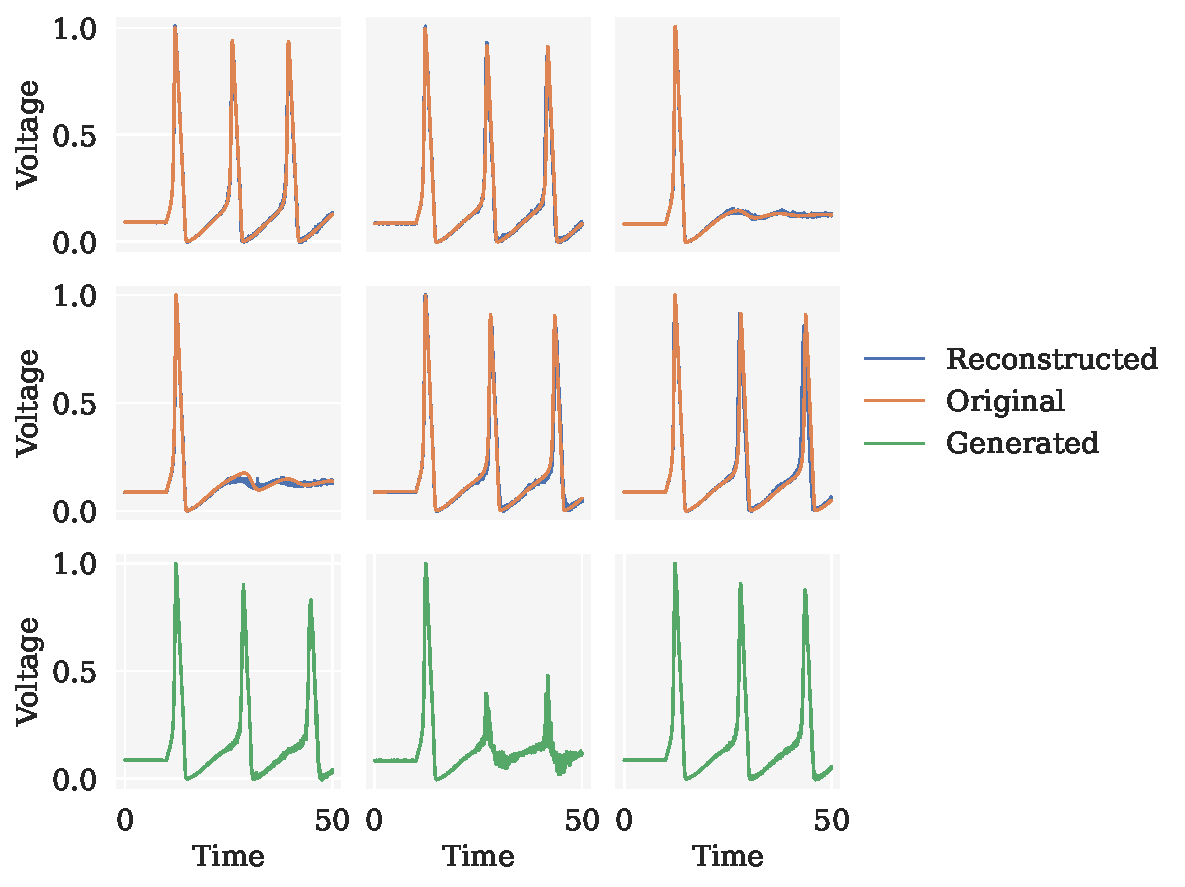
\includegraphics[scale=0.38]{latex/figures/hh_conv_vae_beta_2_z_10.pdf}}}
\qquad
\subfloat[]{{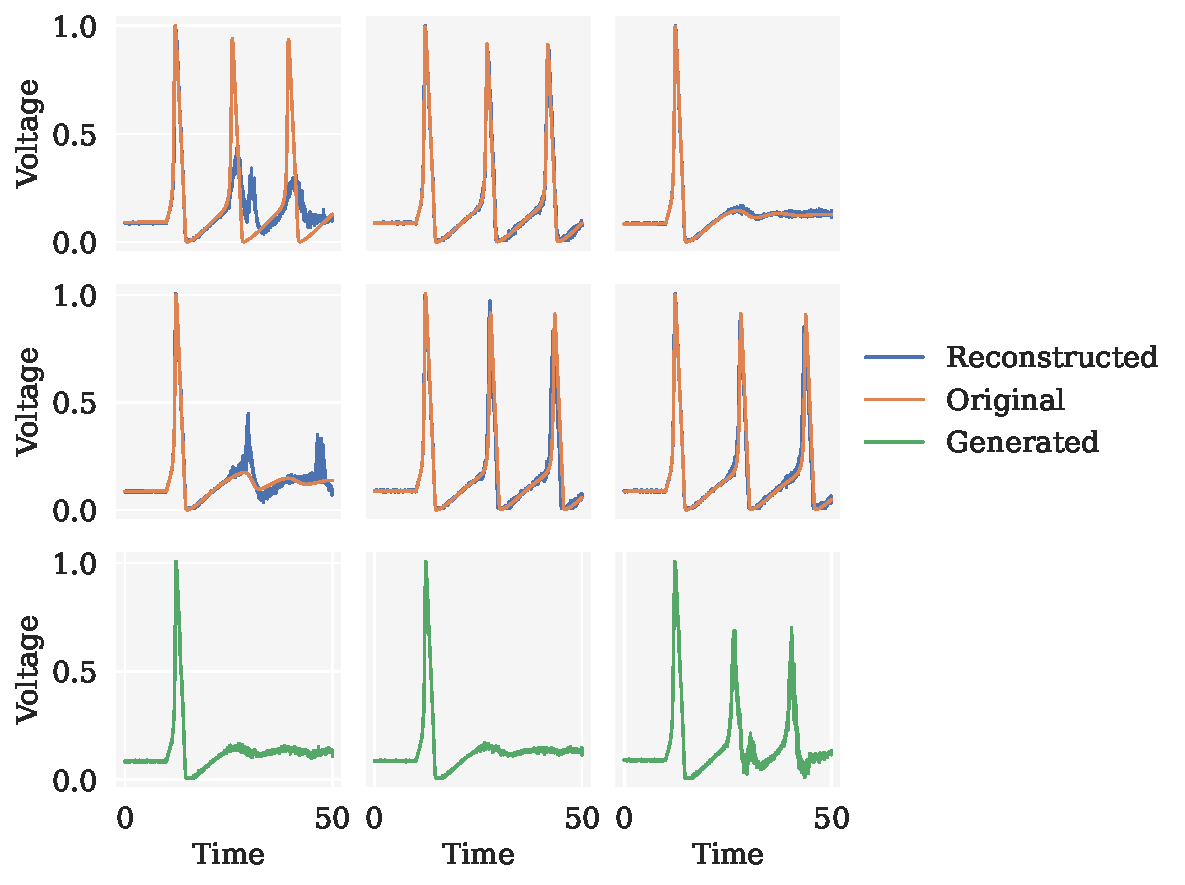
\includegraphics[scale=0.38]{latex/figures/hh_conv_vae_beta_2_z_20.pdf}}}
\caption{Reconstructed voltage traces overlayed with the original signals for a convolutional $\beta$-VAE with $\beta=2$, together with novel voltage traces generated from the latent space. The latent dimensions are (a) 2, (b), 10, (c) 20.}
\label{fig:hh_conv_vae_beta_2}
\end{figure}
